\documentclass{article}

\usepackage{graphicx}
\usepackage{tikz}
\usepackage{tikzsymbols}
\usetikzlibrary{calc,patterns,shapes.geometric}
\pagestyle{empty}
\usepackage[margin=0pt]{geometry}
\geometry{papersize={14in,12in}}

\def\centerarc[#1](#2)(#3:#4:#5){\draw[#1] ($(#2)+({#5*cos(#3)},{#5*sin(#3)})$) arc (#3:#4:#5);}

\begin{document}
	\begin{figure}
		\centering
		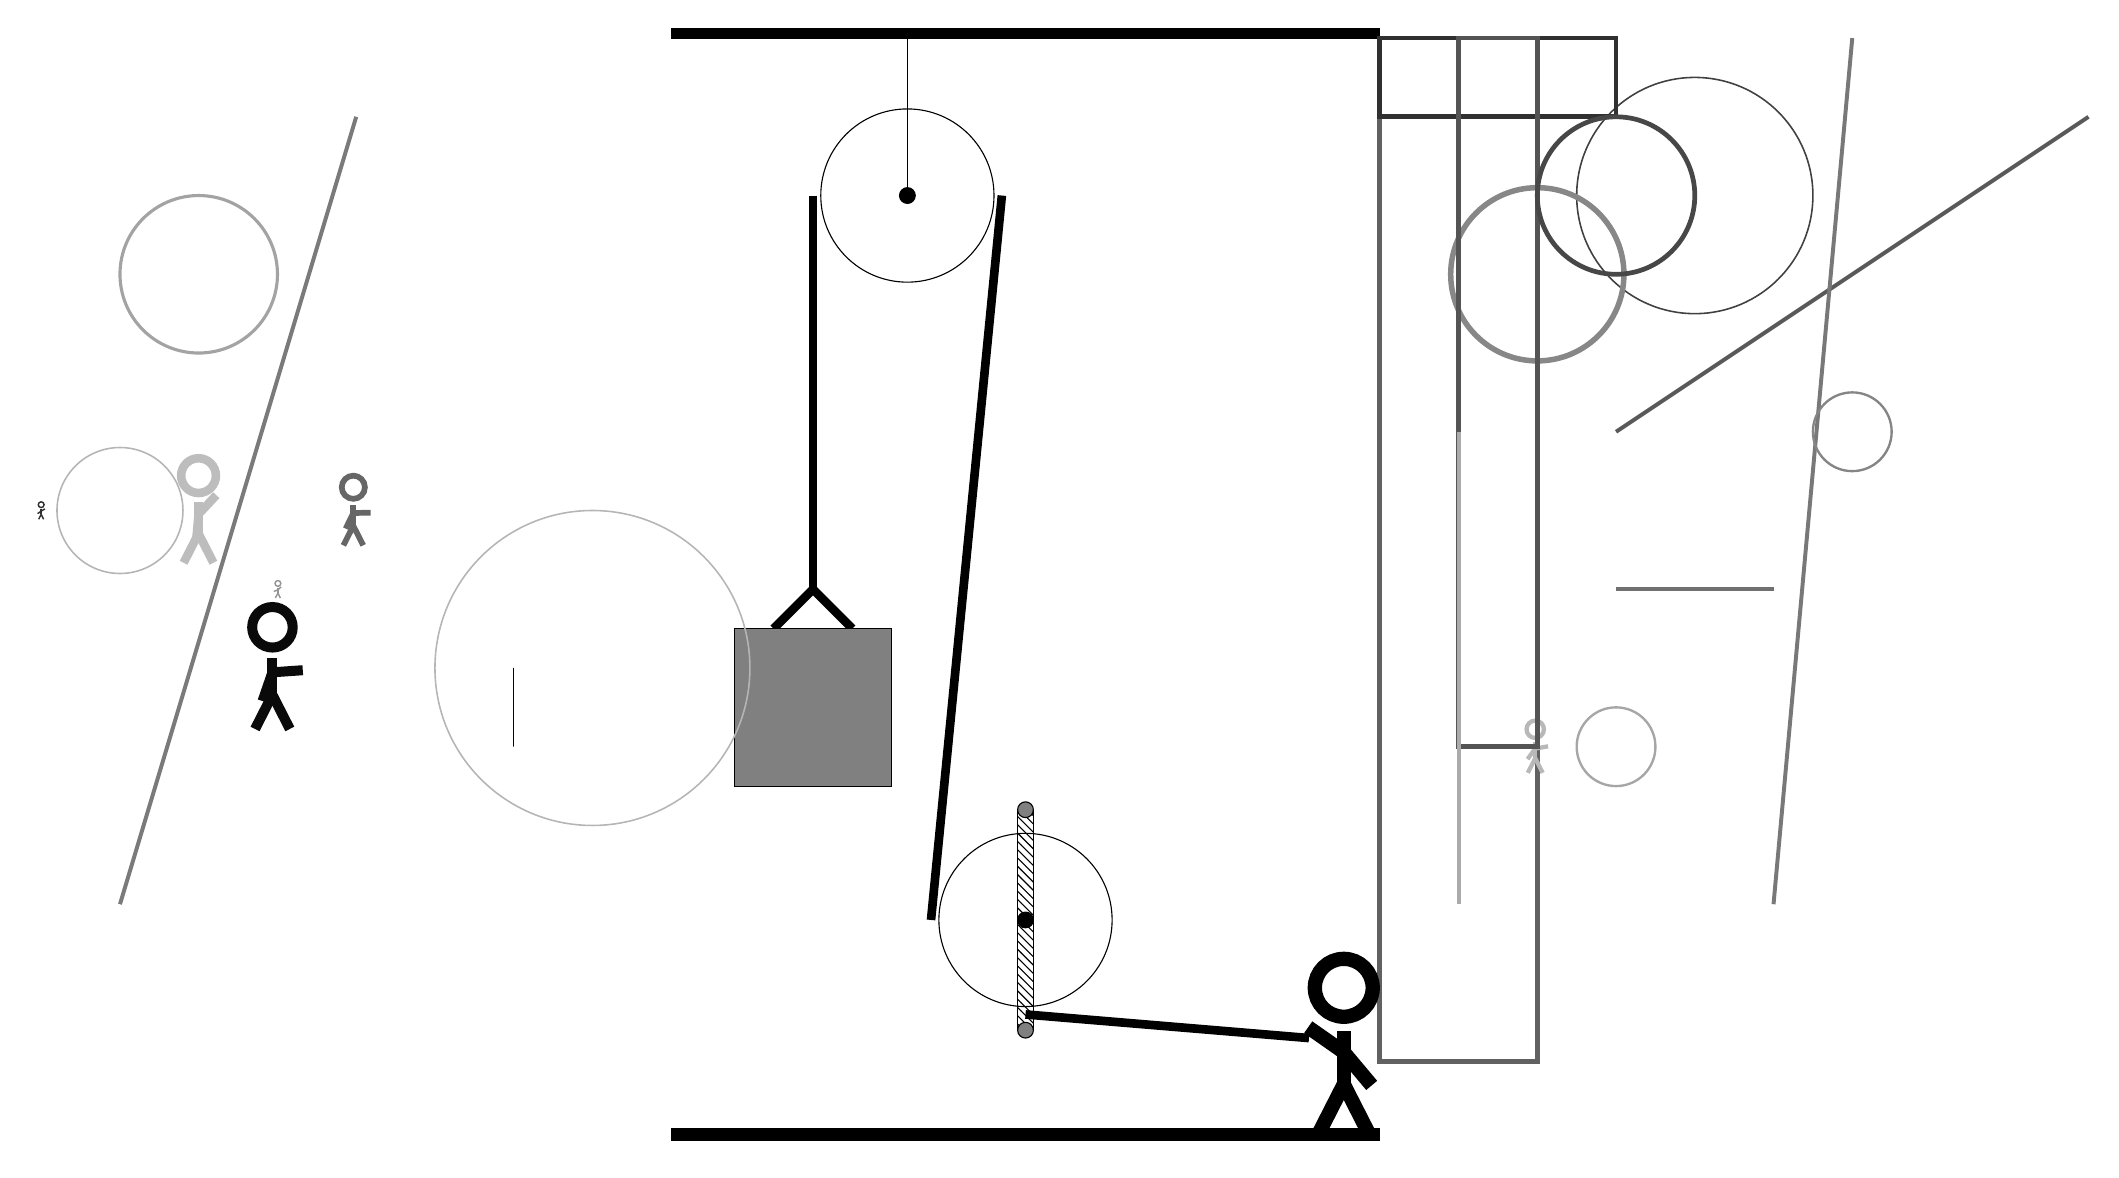
\begin{tikzpicture}
			%%%%% START %%%%%
			
			\draw[fill=black] (-2, 14) rectangle (7, 14.125);
			
			\draw (1, 12) circle (1.1);
			\draw[fill=black] (1, 12) circle (0.1);
			\draw (1, 14) -- (1, 12);
			
			\draw[fill=white](2.5, 2.8) circle (1.1);
			\draw[fill=black] (2.5, 2.8) circle (0.1);
			\draw[pattern=north west lines, pattern color=black] (2.4, 4.2) rectangle (2.6, 1.4);
			\draw[fill=black!50] (2.5, 4.2) circle (0.1);
			\draw[fill=black!50] (2.5, 1.4) circle (0.1);
			
			\draw[line width=1.1mm] (-0.7, 6.5) -- (-0.2, 7.0) -- (0.3, 6.5);
			\draw[fill=black!50] (-1.2, 6.5) rectangle (0.8, 4.5);
			
			\draw [line width=0.2mm, color=black!29](-3, 6) circle (2.0);
			
			\draw [line width=0.2mm, color=black!75](11, 12) circle (1.5);
			\draw [line width=0.7mm, color=black!47](9, 11) circle (1.1);
			\draw[line width=0.6mm, color=black!62] (7, 13) rectangle (9, 1);
			\draw[line width=0.5mm, color=black!56](10, 7) -- (12, 7);
			\draw [line width=0.4mm, color=black!36](-8, 11) circle (1.0);
			
			\node[line width=0.6mm, color=black!60] at (-6, 8) {\Strichmaxerl[4][64][1]};
			\draw[line width=0.5mm, color=black!65](10, 9) -- (16, 13);
			\draw[line width=0.5mm, color=black!52](-6, 13) -- (-9, 3);
			\draw[line width=0.6mm, color=black!81] (7, 13) rectangle (10, 14);
			\draw[line width=0.5mm, color=black!53](12, 3) -- (13, 14);
			\node[line width=0.5mm, color=black!26] at (-8, 8) {\Strichmaxerl[6][85][47]};
			\node[line width=0.7mm, color=black!96] at (-7, 6) {\Strichmaxerl[7][71][4]};
			\node[line width=0.4mm, color=black!28] at (9, 5) {\Strichmaxerl[3][54][10]};
			\node[line width=0.3mm, color=black!82] at (-10, 8) {\Strichmaxerl[1][35][31]};
			\draw[line width=0.6mm, color=black!67] (8, 14) rectangle (9, 5);
			\draw [line width=0.3mm, color=black!35](10, 5) circle (0.5);
			\draw [line width=0.3mm, color=black!48](13, 9) circle (0.5);
			\draw [line width=0.2mm, color=black!29](-9, 8) circle (0.8);
			\draw [line width=0.4mm, color=black!76](-8, 4) circle (0.0);
			\draw[line width=0.2mm, color=black!98] (-4, 5) rectangle (-4, 6);
			
			\node[line width=0.6mm, color=black!42] at (-7, 7) {\Strichmaxerl[1][21][43]};
			\draw [line width=0.6mm, color=black!72](10, 12) circle (1.0);
			\draw[line width=0.5mm, color=black!33](8, 3) -- (8, 9);
			
			\draw[line width=1.1mm] (-0.2, 12) -- (-0.2, 7.0);
			\centerarc[line width=1.1mm](1, 12)(0:180:1.2000000000000002);
			\draw[line width=1.1mm](2.2, 12) -- (1.3, 2.8);
			\centerarc[line width=1.1mm](2.5, 2.8)(180:270:1.2000000000000002);
			\draw[line width=1.1mm](2.5, 1.6) -- (6.1, 1.3);
			
			\node at (6.5, 1.2) {\Strichmaxerl[10][-35][-50]};
			
			\draw[fill=black] (-2, 0) rectangle (7, 0.15);
			
			%%%%% END %%%%%
		\end{tikzpicture}
	\end{figure}	
\end{document}